\section{Appendix}
\label{sec:appendix}


\begin{figure}[H]
\centering
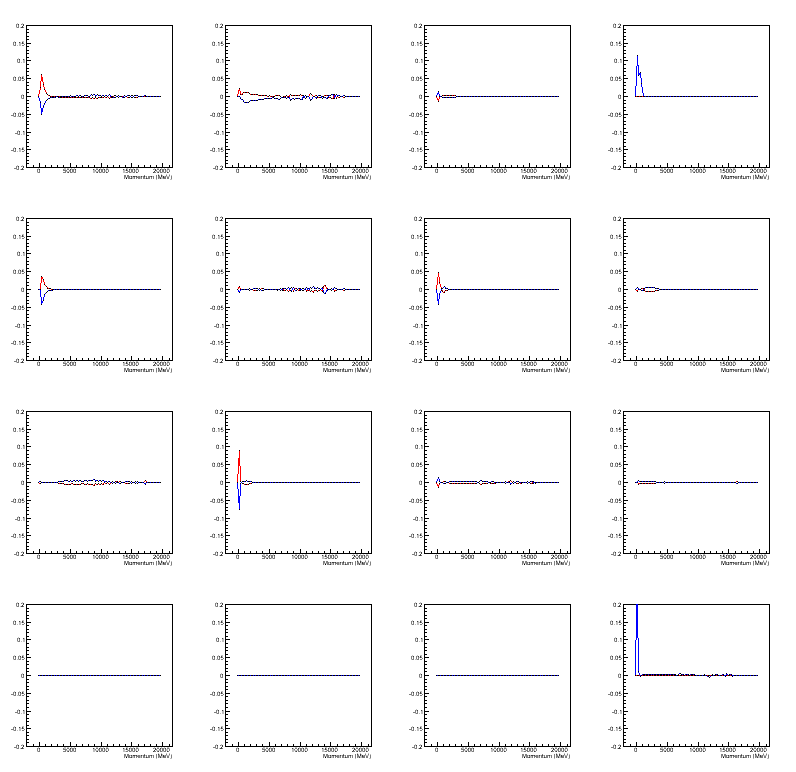
\includegraphics[width=5in]{Figures/TN100Plots/c_7_0.png}
\caption{The fractional change in water-in signal efficiency (predicted from MC) as a function of Muon Momentum for a +1$\sigma$ (blue) and -1$\sigma$ (red) variation of cross section parameter. From left to right, top to bottom, the cross section parameters varied are: MAQE, MARES, DIS Multi-Pi Shape, Spectral Function, Fermi Momentum, Pion-less Delta Decay, CCQE Norm. ($E_\nu < 1.5$GeV), CCQE Norm. ( 3.5~GeV$E_\nu>1.5$GeV), CCQE Norm ($E_\nu > 3.5$GeV), CC 1Pi Norm. ($E_\nu < 2.5$GeV), CC 1Pi Norm. ($E_\nu > 2.5$GeV), CC Coh Norm., NC Coh Norm., NC 1Pi Norm., NC Other Norm., MiniBoone CC 1Pi $E_\nu$ Shape.}
\label{fig:xsvarPwE}
\end{figure}

\begin{figure}[H]
\centering
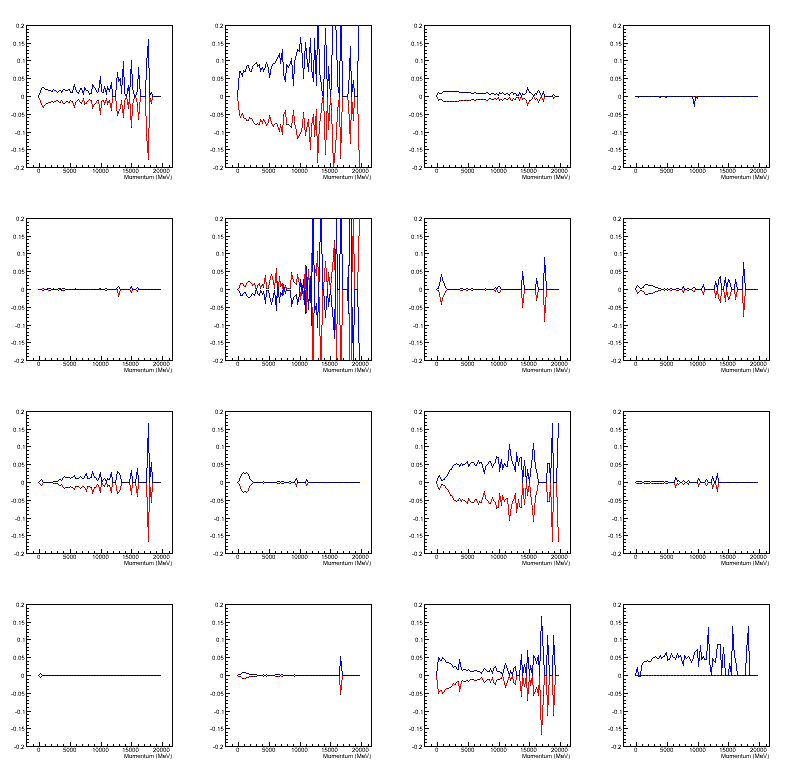
\includegraphics[width=5in]{Figures/TN100Plots/c_13_0.png}
\caption{The fractional change in the water-in background (predicted from MC) as a function of Muon Momentum for a +1$\sigma$ (blue) and -1$\sigma$ (red) variation of cross section parameter. From left to right, top to bottom, the cross section parameters varied are: MAQE, MARES, DIS Multi-Pi Shape, Spectral Function, Fermi Momentum, Pion-less Delta Decay, CCQE Norm. ($E_\nu < 1.5$GeV), CCQE Norm. ( 3.5~GeV$E_\nu>1.5$GeV), CCQE Norm ($E_\nu > 3.5$GeV), CC 1Pi Norm. ($E_\nu < 2.5$GeV), CC 1Pi Norm. ($E_\nu > 2.5$GeV), CC Coh Norm., NC Coh Norm., NC 1Pi Norm., NC Other Norm., MiniBoone CC 1Pi $E_\nu$ Shape.}
\label{fig:xsvarPwB}
\end{figure}

\begin{figure}[H]
\centering
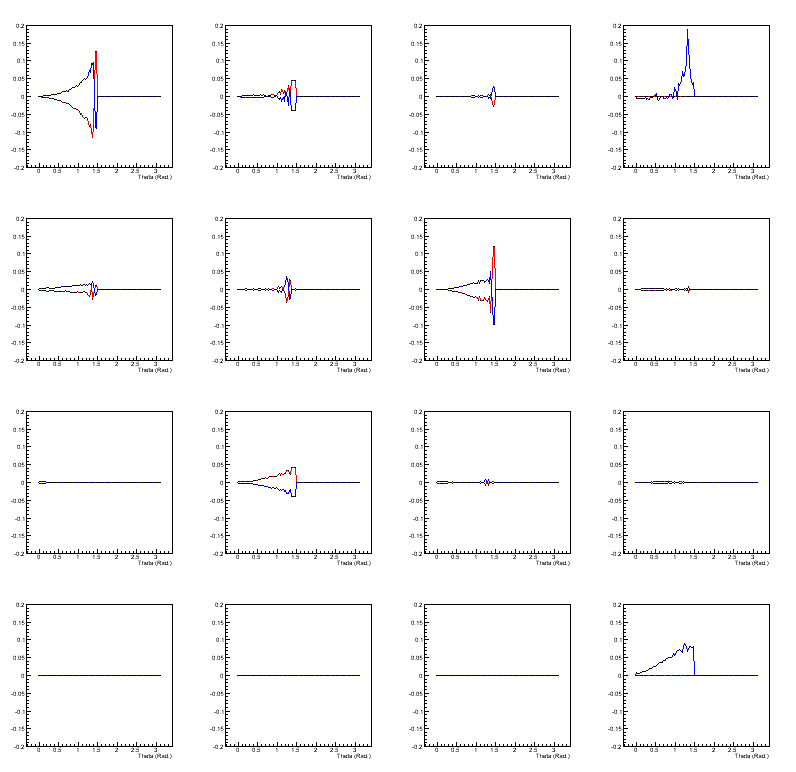
\includegraphics[width=5in]{Figures/TN100Plots/c_8_0.png}
\caption{The fractional change in the water-in signal efficiency (predicted from MC) as a function of Muon Track Theta for a +1$\sigma$ (blue) and -1$\sigma$ (red) variation of cross section parameter. From left to right, top to bottom, the cross section parameters varied are: MAQE, MARES, DIS Multi-Pi Shape, Spectral Function, Fermi Momentum, Pion-less Delta Decay, CCQE Norm. ($E_\nu < 1.5$GeV), CCQE Norm. ( 3.5~GeV$E_\nu>1.5$GeV), CCQE Norm ($E_\nu > 3.5$GeV), CC 1Pi Norm. ($E_\nu < 2.5$GeV), CC 1Pi Norm. ($E_\nu > 2.5$GeV), CC Coh Norm., NC Coh Norm., NC 1Pi Norm., NC Other Norm., MiniBoone CC 1Pi $E_\nu$ Shape.}
\label{fig:xsvarTwE}
\end{figure}

\begin{figure}[H]
\centering
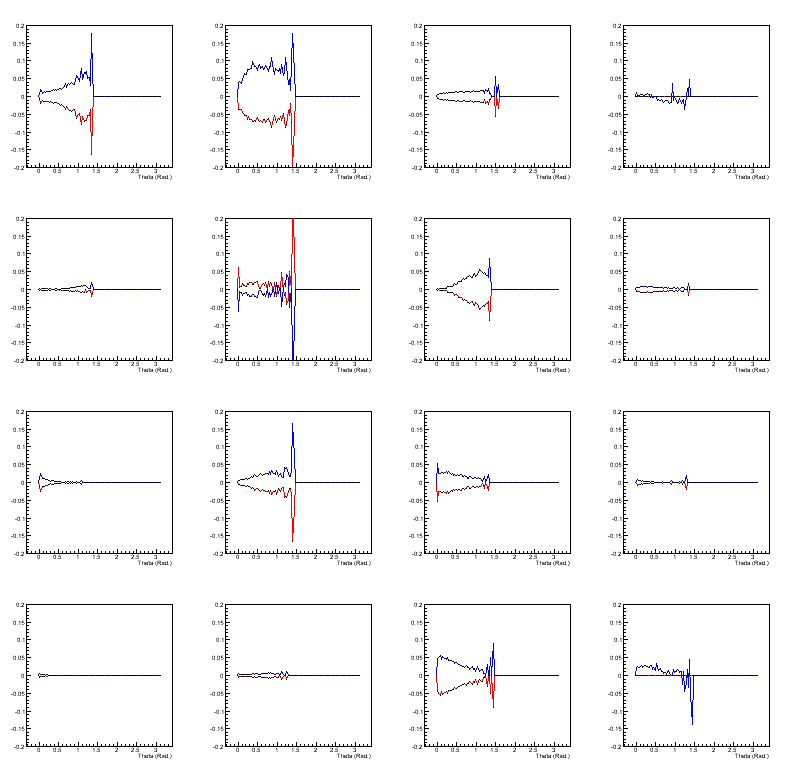
\includegraphics[width=5in]{Figures/TN100Plots/c_14_0.png}
\caption{The fractional change in the water-in background (predicted from MC) as a function of Muon Track Theta for a +1$\sigma$ (blue) and -1$\sigma$ (red) variation of cross section parameter. From left to right, top to bottom, the cross section parameters varied are: MAQE, MARES, DIS Multi-Pi Shape, Spectral Function, Fermi Momentum, Pion-less Delta Decay, CCQE Norm. ($E_\nu < 1.5$GeV), CCQE Norm. ( 3.5~GeV$E_\nu>1.5$GeV), CCQE Norm ($E_\nu > 3.5$GeV), CC 1Pi Norm. ($E_\nu < 2.5$GeV), CC 1Pi Norm. ($E_\nu > 2.5$GeV), CC Coh Norm., NC Coh Norm., NC 1Pi Norm., NC Other Norm., MiniBoone CC 1Pi $E_\nu$ Shape.}
\label{fig:xsvarTwB}
\end{figure}

\begin{figure}[H]
\centering
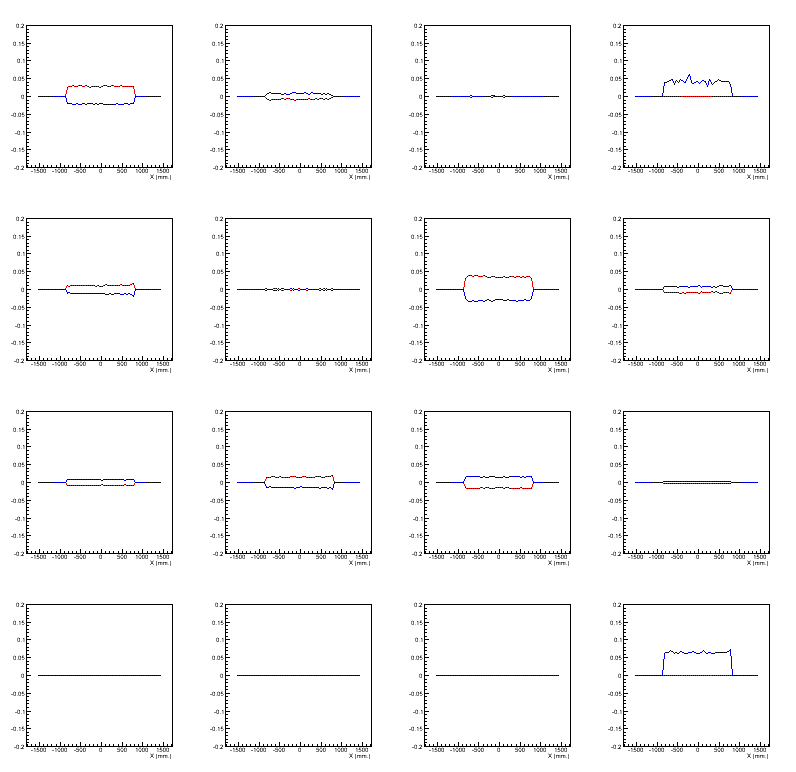
\includegraphics[width=5in]{Figures/TN100Plots/c_9_0.png}
\caption{The fractional change in the water-in signal efficiency (predicted from MC) as a function of X position of the vertex for a +1$\sigma$ (blue) and -1$\sigma$ (red) variation of cross section parameter. From left to right, top to bottom, the cross section parameters varied are: MAQE, MARES, DIS Multi-Pi Shape, Spectral Function, Fermi Momentum, Pion-less Delta Decay, CCQE Norm. ($E_\nu < 1.5$GeV), CCQE Norm. ( 3.5~GeV$E_\nu>1.5$GeV), CCQE Norm ($E_\nu > 3.5$GeV), CC 1Pi Norm. ($E_\nu < 2.5$GeV), CC 1Pi Norm. ($E_\nu > 2.5$GeV), CC Coh Norm., NC Coh Norm., NC 1Pi Norm., NC Other Norm., MiniBoone CC 1Pi $E_\nu$ Shape.}
\label{fig:xsvarXwE}
\end{figure}

\begin{figure}[H]
\centering
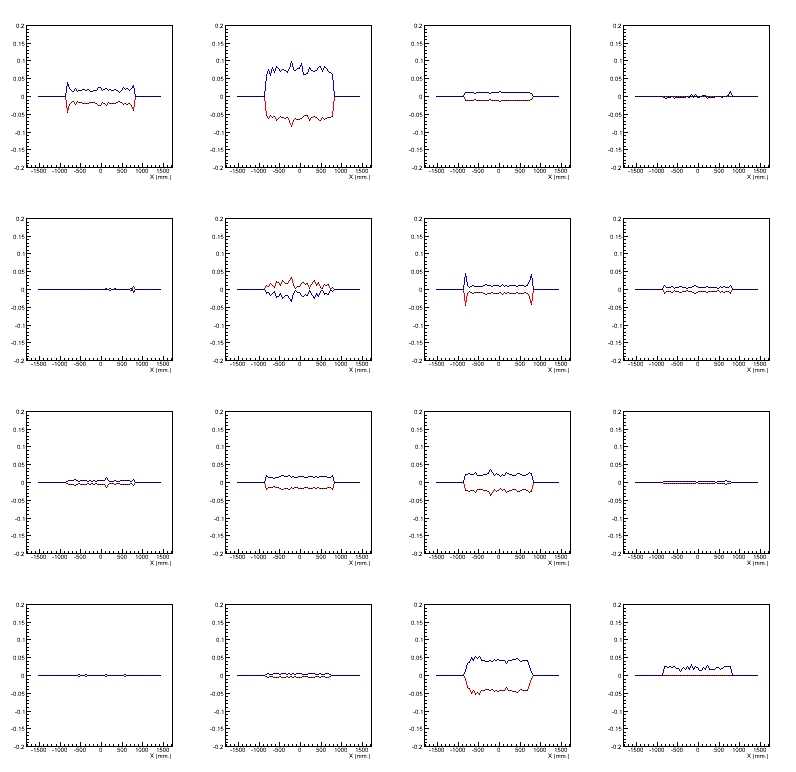
\includegraphics[width=5in]{Figures/TN100Plots/c_15_0.png}
\caption{The fractional change in the water-in background (predicted from MC) as a function of X position of the vertex for a +1$\sigma$ (blue) and -1$\sigma$ (red) variation of cross section parameter. From left to right, top to bottom, the cross section parameters varied are: MAQE, MARES, DIS Multi-Pi Shape, Spectral Function, Fermi Momentum, Pion-less Delta Decay, CCQE Norm. ($E_\nu < 1.5$GeV), CCQE Norm. ( 3.5~GeV$E_\nu>1.5$GeV), CCQE Norm ($E_\nu > 3.5$GeV), CC 1Pi Norm. ($E_\nu < 2.5$GeV), CC 1Pi Norm. ($E_\nu > 2.5$GeV), CC Coh Norm., NC Coh Norm., NC 1Pi Norm., NC Other Norm., MiniBoone CC 1Pi $E_\nu$ Shape.}
\label{fig:xsvarXwB}
\end{figure}

\begin{figure}[H]
\centering
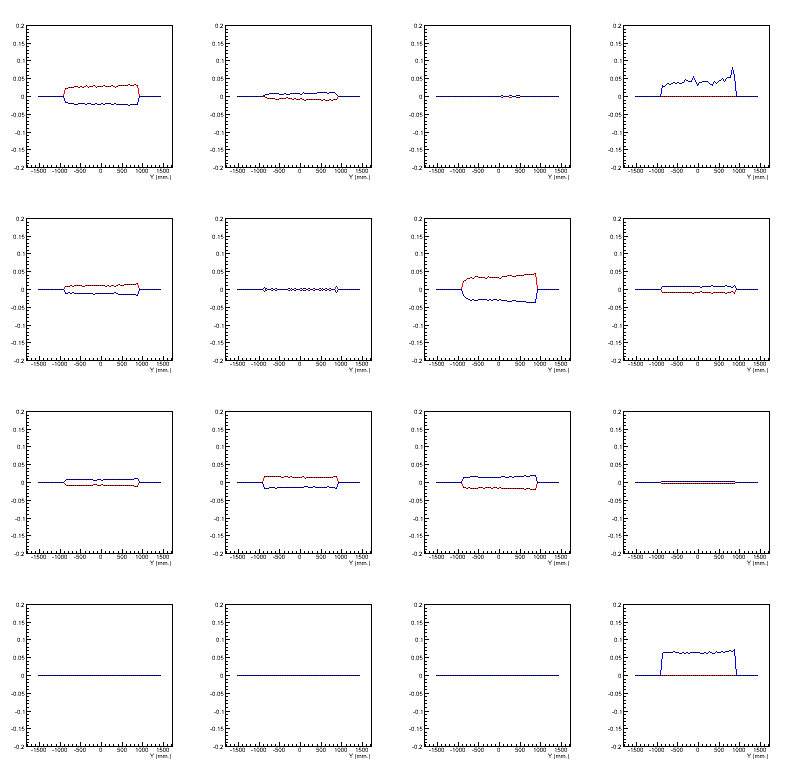
\includegraphics[width=5in]{Figures/TN100Plots/c_10_0.png}
\caption{The fractional change in the water-in signal efficiency (predicted from MC) as a function of Y position of the vertex for a +1$\sigma$ (blue) and -1$\sigma$ (red) variation of cross section parameter. From left to right, top to bottom, the cross section parameters varied are: MAQE, MARES, DIS Multi-Pi Shape, Spectral Function, Fermi Momentum, Pion-less Delta Decay, CCQE Norm. ($E_\nu < 1.5$GeV), CCQE Norm. ( 3.5~GeV$E_\nu>1.5$GeV), CCQE Norm ($E_\nu > 3.5$GeV), CC 1Pi Norm. ($E_\nu < 2.5$GeV), CC 1Pi Norm. ($E_\nu > 2.5$GeV), CC Coh Norm., NC Coh Norm., NC 1Pi Norm., NC Other Norm., MiniBoone CC 1Pi $E_\nu$ Shape.}
\label{fig:xsvarYwE}
\end{figure}

\begin{figure}[H]
\centering
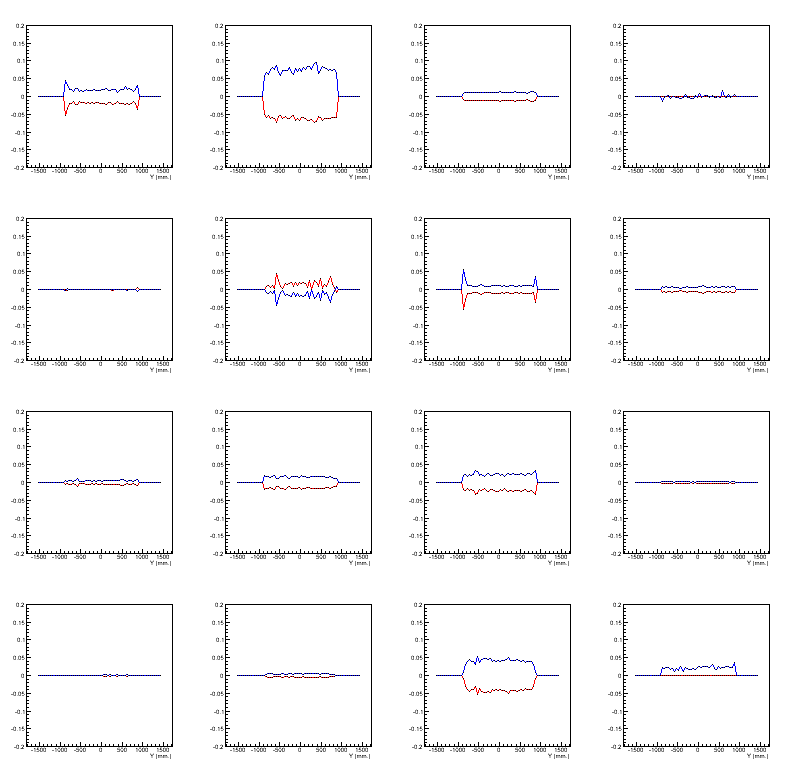
\includegraphics[width=5in]{Figures/TN100Plots/c_16_0.png}
\caption{The fractional change in the water-in background (predicted from MC) as a function of Y position of the vertex for a +1$\sigma$ (blue) and -1$\sigma$ (red) variation of cross section parameter. From left to right, top to bottom, the cross section parameters varied are: MAQE, MARES, DIS Multi-Pi Shape, Spectral Function, Fermi Momentum, Pion-less Delta Decay, CCQE Norm. ($E_\nu < 1.5$GeV), CCQE Norm. ( 3.5~GeV$E_\nu>1.5$GeV), CCQE Norm ($E_\nu > 3.5$GeV), CC 1Pi Norm. ($E_\nu < 2.5$GeV), CC 1Pi Norm. ($E_\nu > 2.5$GeV), CC Coh Norm., NC Coh Norm., NC 1Pi Norm., NC Other Norm., MiniBoone CC 1Pi $E_\nu$ Shape.}
\label{fig:xsvarYwB}
\end{figure}
